\begingroup
\hyphenpenalty=10000\exhyphenpenalty=10000
\definecolor{IEEEBlue}{HTML}{00629B}\definecolor{Cyan}{HTML}{00A6B2}
\definecolor{Navy}{HTML}{003B5C}\definecolor{Slate}{HTML}{526470}
\definecolor{BridgeRed}{HTML}{B83136}\definecolor{BridgeAmber}{HTML}{A66610}
\definecolor{BridgeGreen}{HTML}{287449}
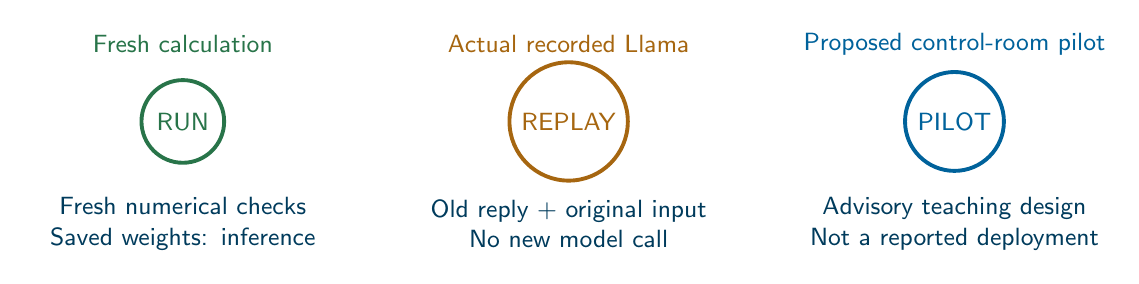
\begin{tikzpicture}[x=1cm,y=1cm,font=\sffamily\fontsize{9}{11}\selectfont,
every node/.style={text=Navy},
flow/.style={-{Stealth[length=2mm]},draw=IEEEBlue,line width=1.1pt},
muted/.style={draw=Slate!55,line width=.6pt},
bridgebox/.style={draw=IEEEBlue,line width=.85pt,fill=white,align=center,minimum height=.9cm,inner sep=5pt},
plain/.style={align=center,inner sep=2pt},
small/.style={font=\sffamily\fontsize{8.5}{10.5}\selectfont},
stop/.style={draw=BridgeRed,fill=BridgeRed!4,text=BridgeRed,line width=1pt,align=center,minimum height=.9cm,inner sep=5pt}]

\node[circle,draw=BridgeGreen,line width=1.4pt,text=BridgeGreen,minimum size=1.05cm] at (2.2,2.2) {RUN};
\node[plain,text=BridgeGreen] at (2.2,3.18) {Fresh calculation};
\node[plain,text width=3.8cm] at (2.2,.9) {Fresh numerical checks\\Saved weights: inference};
\node[circle,draw=BridgeAmber,line width=1.4pt,text=BridgeAmber,minimum size=1.05cm] at (7.1,2.2) {REPLAY};
\node[plain,text=BridgeAmber] at (7.1,3.18) {Actual recorded Llama};
\node[plain,text width=3.8cm] at (7.1,.9) {Old reply + original input\\No new model call};
\node[circle,draw=IEEEBlue,line width=1.4pt,text=IEEEBlue,minimum size=1.05cm] at (12.0,2.2) {PILOT};
\node[plain,text=IEEEBlue] at (12.0,3.18) {Proposed control-room pilot};
\node[plain,text width=3.8cm] at (12.0,.9) {Advisory teaching design\\Not a reported deployment};
\end{tikzpicture}
\endgroup
